% Standalone source for the manuscript's Figure 1 (tolerance corridor).
% Compile: pdflatex fig3_anchor_corridor_standalone.tex
\documentclass[border=2pt]{standalone}
\usepackage[T1]{fontenc}
\usepackage{lmodern}
\usepackage{graphicx}
\usepackage{tikz}
\usetikzlibrary{arrows.meta}
\begin{document}
\resizebox{0.72\textwidth}{!}{%
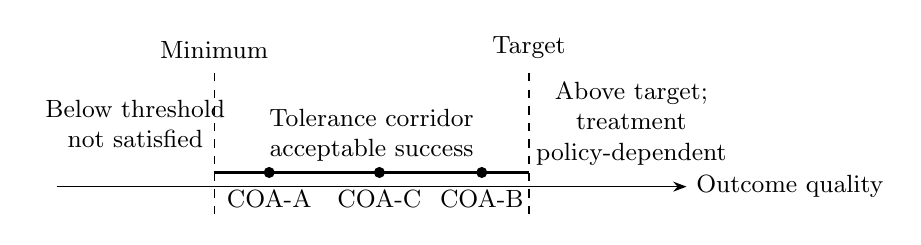
\begin{tikzpicture}[>=Stealth, every node/.style={font=\small}]
\draw[->] (0,0) -- (8,0) node[right]{Outcome quality};
\draw[very thick] (2,0.18) -- (6,0.18);
\draw[dashed] (2,-0.35) -- (2,1.5) node[above]{Minimum};
\draw[dashed] (6,-0.35) -- (6,1.5) node[above]{Target};
\node[align=center] at (4,0.65) {Tolerance corridor\\acceptable success};
\fill (2.7,0.18) circle (2pt) node[below=3pt]{COA-A};
\fill (4.1,0.18) circle (2pt) node[below=3pt]{COA-C};
\fill (5.4,0.18) circle (2pt) node[below=3pt]{COA-B};
\node[align=center, text width=2.5cm] at (1.0,0.8) {Below threshold\\not satisfied};
\node[align=center, text width=2.6cm] at (7.3,0.8) {Above target;\\treatment\\policy-dependent};
\end{tikzpicture}}
\end{document}
